\chapter{Theoretical Background}

This chapter explains the concepts needed to understand this thesis. The theory behind RL, ANN, DDPG and HER is explained.

\section{Reinforcement Learning}
%% In context of machine learning (supervised,unsupervised)
%% potential to be better than humans

RL is one of the main learning concepts of Machine Learning next to Supervised Learning and Unsupervised Learning \cite{machinelearning}.
\newline
In Supervised Learning some input data is given to the learning agent. The agent is expected to come up with some output which is then compared with the expected output. If the output given by the agent and the expected output matches, then the agent was correct. The agent is trained by calculating the error between expected output and actual output. An use case for Supervised Learning is sorting mails into regular mail and spam mail. The agent is given a mail and it should decide whether the mail is regular or spam based on the content. Supervised Learning is used for classification and regression problems \cite{machinelearning}. It is mainly useful when the expected output is already known, so the learning agent can learn to do recognize these. 
\newline
In Unsupervised Learning there is no expected output. The learning agent is fed with data so it can figure out interesting features and similarities between different data. Unsupervised Learning is often used to cluster data, often pictures, based on similarities \cite{machinelearning}.
\newline
In RL the agent is learning through rewards that are given through interaction with an environment. The goal of a task is clear, but the path of actions to reach the goal is not trivial. RL is used to find the best action in each situation. It is often used for games because they are already set up to have a clear task and goal, but the optimal way to reach it is not clear. Games usually provide full information on the environment in contrast to the real world, therefore setting up the learning environment is simple. Also Supervised Learning is limited in performance because the agent can only learn to become as good the expected output that we set. So in games like chess, with Supervised Learning the agent can only become as good as the best players it learns from, but not better. It is limited by the skills of the best humans \cite{nolimit}. However, RL is not restricted by these limitations. The agent can improve on its own only by exploring his options. In games like Go and Chess, engines that use RL have already far surpassed the best human players \cite{alphazero}. 

\vspace{0.5cm}

%%general idea
This section will explain the theory behind RL. The post by Lilian Weng is recommended as a resource on more precise explanations on RL \cite{rllilianweng}. RL is usually modeled as a Markov Decision Process. The Markov Decision Process for RL consists of following elements \cite{rlwiki}:

\begin{itemize}
	\item A set of states S
	\item A set of actions A
	\item The transition probability $P_a(s,s')$ from state s to s' under action a
	\item The immediate reward $R_a(s,s')$ of that transition
	\item rules that describe the agents observation
\end{itemize}

The agent and environment are in a state s. The agent chooses an action a from its set of possible actions A to interact with the environment. The environment reacts by transitioning to another state and returning a reward R and an observation to the agent. Depending on the model the transitions might be stochastic or deterministic. The aim of the agent is to earn the maximal total reward possible. In order to reach this aim, the agent interacts with the environment to gain knowledge about the environment through the gained rewards and observations. Through this process, the agent learns in which state which actions are better to gain more reward. This is illustrated by Figure \ref{rl_general}.

\begin{figure} [h]
	
	\centering
	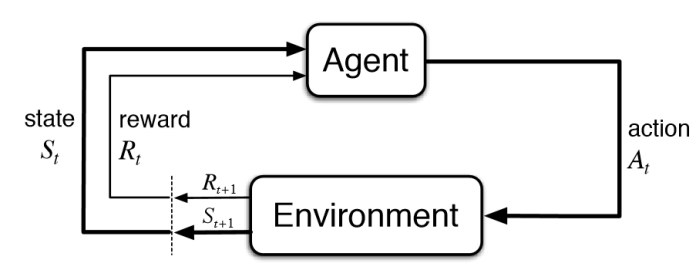
\includegraphics[width=1\textwidth]{figures/rl_general.jpg}
	\caption{Reinforcement Learning. An agent chooses an action to interact with the environment and gets a reward and an observation of his new state back. 
		\label{rl_general}	
		\cite{rl_general.jpg}
	}
\end{figure}

\vspace{0.5cm}

%policy 
In each state there is an action that the agent considers best due to its current knowledge about the expected rewards of each action. This set of actions is known as the policy 
$\pi (s)$. 
The goal of getting maximal reward can be interpreted as finding the best actions in each state that give the most reward, which is finding the optimal policy. The policy can also be either deterministic or stochastic, depending on the transition probability of the environment.

\vspace{0.5cm}

%value function
A value function is used to measure how good a state or action is. Two types of value functions are used for the states and the actions. the state value function is denoted as V(s). The value of a state is the expected reward when acting according to the policy 
$\pi$ \cite{rlwiki}.
V(s) is defined as follows in equation \ref{eq:state-value-function}.

\begin{equation}
\label{eq:state-value-function}
V^\pi (s) = \mathbb{E} [R | s,\pi]
\end{equation}

The actions value function is denoted as Q(s,a) and is defined In equation \ref{eq:action-value-function}.

\begin{equation}
\label{eq:action-value-function}
Q^\pi (s,a) = \mathbb{E} [R | s,a,\pi]
\end{equation}

When determining the value of a state or action, a discount factor $\gamma$
is used to discount future rewards towards immediate rewards. 
The idea is that a state s is not only as good as the reward you get when transitioning to that state. Future rewards from states that are reachable from state s should also be considered. The value of a state consists of the reward that you get by transitioning to that state and the potential rewards that can be gained by transitioning from that state. 
Since future rewards are not as certain as immediate rewards, the discount factor is used. The farther a reward is in the future, the more it is discounted. 
%bellman equations
The Bellman equations described in equation \ref{eq:V-bellman} and \ref{eq:Q-bellman} are a set of equations that convert the value functions into the immediate and future reward and can be used to update the value-functions \cite{rllilianweng}.

\begin{equation}
\label{eq:V-bellman}
V_\pi (s) = \sum_{a \in A}  \pi(a|s) (R(s,a) + \gamma \sum_{s' \in S} P_{ss'}^a V_\pi (s'))
\end{equation}

\begin{equation}
\label{eq:Q-bellman}
Q_\pi (s,a) = R(s,a) + \gamma \sum_{s' \in S} P_{ss'}^a \sum_{a \in A}  \pi(a'|s') Q_\pi(s',a')
\end{equation}

The goal is to find the actions that return the maximal reward. This is displayed by the Bellman optimality equations (\ref{eq:V-optbellman},\ref{eq:Q-optbellman}) \cite{rllilianweng}:

\begin{equation}
\label{eq:V-optbellman}
V_\ast (s) = \max_{a \in A} (R(s,a) + \gamma \sum_{s' \in S} P_{ss'}^a V_\ast (s'))
\end{equation}

\begin{equation}
\label{eq:Q-optbellman}
Q_\ast (s,a) = R(s,a) + \gamma \sum_{s' \in S} P_{ss'}^a \max_{a \in A} Q_\ast(s',a')
\end{equation}

To calculate the optimal values of each state and action, Dynamic Programming could be used if the entire model is known. But even knowing the entire model is not good enough as usually the main issue lies in the huge state and action space, which makes it impossible to use Dynamic Programming. For RL, artificial neural networks (ANNs) can be used to approximate the value functions \cite{neuralnetpath}. 

When following the current policy, the agent will earn the maximal reward that it could earn with current knowledge, but never more than that. To learn, the agent has to deviate from the policy and explore different actions and states. The question is how much deviation is necessary, as the agent also needs to exploit most of the policy path it has learned until now because following most of the policy has a higher probability of earning a high reward. This is known in RL as the exploration vs. exploitation problem. Usually there is a variable $\epsilon$ that determines with which probability the agent will deviate from the policy. It is set rather low to let the agent exploit most of its policy. As an example, an approach is $\epsilon$-greedy \cite{egreedy}. With a high probability of $1-\epsilon$ the agent will choose the policy and with a probability of $\epsilon$ a random action is chosen. This ensures that the agent exploits most of the policy, but also explores more possible actions that might bring more reward. 

%%neuronal networks
\section{Artificial Neural Networks}

ANNs are inspired by the human brain. 
%\nnbio, blablabla
The ANN consists of layers of neurons. Each neuron is connected to the next layer of neurons. There is one input layer and one output layer at the beginning and end of the layer of neurons. The layers between the input and output layers are called hidden layer. The hidden layer can consist of only one or more layers. The idea is to train the ANN to take inputs and produce outputs. To approximate the value functions the input would be states and actions, the output should be the correct and optimal values of these states and actions. An example of an ANN is shown in Figure \ref{neuralnet}.

\begin{figure} [h]
	\centering
	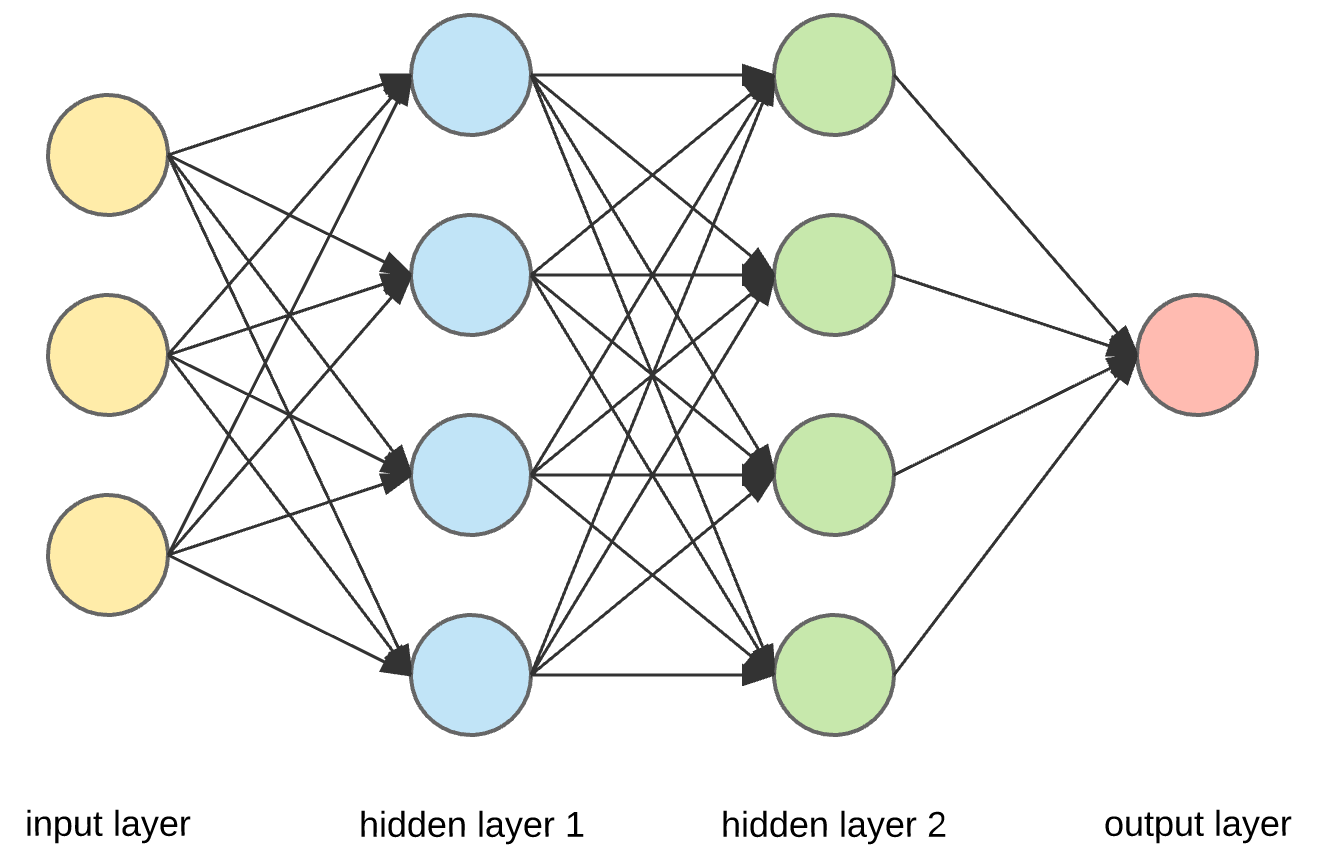
\includegraphics[width=1\textwidth]{figures/neural_network.png}
	\caption{A neural network. \cite{neural_networkpng}}
	\label{neuralnet}
\end{figure}

\vspace{0.5cm}

The learning process of the neuronal network is as follows. Each neuron obtains inputs $x_i$ by the the outputs of the neurons in the layer before it. Each input value is weighted and then the sum of these weighted values is taken. A bias $b$ is also added to support the learning process. After using an activation function on the sum, the value is output to the next layer of neurons. The activation function is a simple function that either reduces the output of the neuron to 0 if the value is below a certain threshold, otherwise the value is output unfiltered.
The training process of the neuron can be seen in Figure \ref{neuron}.
%besser formulieren!

\begin{figure} [h]	
	\centering
	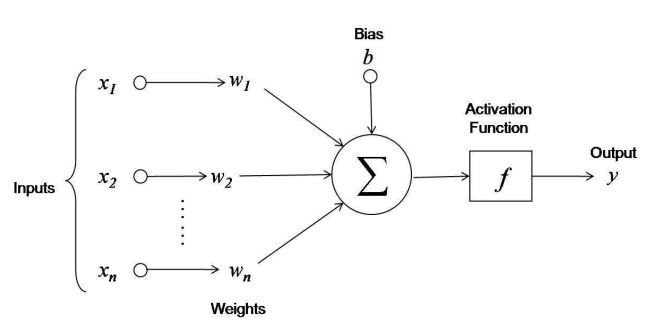
\includegraphics[width=1\textwidth]{figures/neuron.jpeg}
	\caption{A neuron and how its value is composed \cite{neuron.jpeg}}
	\label{neuron}
\end{figure}

\vspace{0.5cm}

When the ANN outputs a value, a process called Backpropagation is used to improve the ANN \cite{backprop}. When initializing the ANN, the actual right weights for the input values are unknown, so random values for the weights are used. Therefore, the output values will not be right. By using an error function, the amount of error can be computed. The amount of error can be used to figure out how much the weights have to be modified for the output to become right. Backpropagation is the process of going backwards through the ANN and improving the weights of the neurons that caused the output value to be wrong. By repeating the whole process, the weight of each neuron converges towards an optimal value. 

\vspace{0.5cm}

\section{Deep Deterministic Policy Gradients}

The paper by Silver et al. is a recommended resource for more detailed explanations \cite{ddpg}. This chapter will give a short summary of DDPG.
The algorithm DDPG learns concurrently a Q-function (the action-value function) and a policy. \cite{ddpg}
Q*(s,a) is used to find the the optimal action in each state.
To compute the Q-values for a discrete action space, the Q-values of each action could be calculated and compared to find the biggest value. But in a continuous action space it is not possible to calculate the Q-value for each action. DDPG uses the fact that the action space is continuous and so Q*(s,a) is expected to be differentiable in respect to the action argument. \cite{ddpg}
This way it is possible to approximate the Q-values and policy.

\vspace{0.5cm}

To learn the Q-values, the Bellman equation for the action value is used. To approximate the Q-values, a mean squared Bellman error function is used.
The idea is that minimizing this function error is equal to approximating the current Q-values to the optimal Q-values.

\vspace{0.5cm}

For DDPG an experience replay buffer is also used. The replay buffer is a set of experiences. This can be used to replay old experiences. When only using new experiences, the ANN might be overfit to those experiences. Being overfit means that for some experiences the ANN will output very good results, but for most other experiences it will perform very bad. Experience replay is useful to prevent that. But a too large buffer can cause the learning process to slow down. The right balance has to be found.

DDPG also uses target networks. Equation \ref{eq:target} is called target \cite{ddpg}.

\begin{equation}
\label{eq:target}
r + \gamma (1-d) \max_{a'} Q_\phi(s',a')
\end{equation}

The target is what is desired for the Q-function to approximate to.
When minimizing the mean squared bellman error function, there is the problem that the target is also dependent on the parameters that are trained. When changing the parameters, the target would also change which is problematic. That is why the target network, a copy of the ANN is used. The update of the target network is delayed to avoid this conflict.
To find the optimal policy, simply gradient ascent can be used to find the maximal Q-values.


\section{Hindsight Experience Replay}

%subsection curriculum learning ?

%read paper, use it
Sparse rewards are a big issue in RL, especially in tasks for robotic arms often the rewards are sparse. Having sparse rewards means that most of the samples used for training will not successful and therefore will not bring any useful reward. For example, the task to move an object to a certain point would have a sparse reward for a robotic arm because very precise movements are needed which the robotic arm has to learn first.
 
\vspace{0.5cm}
 
Andrychowicz et al. have shown that HER can be used to deal with this issue for robotic arms \cite{herpaper}
HER can learn efficiently from sparse rewards and can also be combined with any off-policy RL algorithm.
This technique is inspired by the ability of humans to learn from failures as least as much as from successes.

\vspace{0.5cm}

HER works as follows. After an episode of gaining experiences, all transitions between the states in each training sample is stored in a replay buffer, but the goal that was not achieved is extended to a set with a goal that is reached. This can also be further extended to a set of more goals that can be achieved in the terminating state of the training sample. If the goal was to move an object to point x, but it was pushed to point y, the replay buffer would use the same transitions but change the the goal we wanted to achieve to y. So when replaying the same experience, the agent would be successful and earn an useful reward. This does not help the agent learn how to reach the goal it wanted to reach initially, but it learns how to reach other goals. Being able to reach those other already achieved goals might be beneficial in learning how to reach the goal it actually wanted to achieve. HER is mainly used for tasks with multiple goals, but it was shown that it also improves the training of tasks with only a single goal. \cite{herpaper}
Interestingly, Andrychowicz et al. have shown HER performs has problems when using shaped rewards. \cite{herpaper}
%add binary rewards at start of section ?. binary != shaped ?
 
 %add pseudocode ?
